\textbf{COLUNI 2026 -- Questão 38}\par\medskip O trecho a seguir é parte de uma longa entrevista cedida ao Museu da Imagem e do Som (MIS) do Rio de Janeiro, em 1968, por João Cândido, que liderou um movimento na Primeira República (1889-1930), no Brasil, e ficou conhecido por muitos como “Almirante Negro”.

\begin{minipage}{0.43\linewidth}
“Eu tive o poder na organização da conspiração e estive determinado pelos comitês para assumir a direção da revolução com todos os poderes [...]. Assumi a liderança já indicado pelos demais comitês. Houve a formação dos grupos, cada grupo tinha sua função [...]. Nós tínhamos nossos próprios especialistas, que estudaram [...] o movimento [...] a fundo [...].”\par
BRAICK, Patrícia Ramos. Estudar história: das origens do homem à era digital. São Paulo: Moderna, 2015, 9º ano, p.43.\par
Ao lado, João Cândido, à direita da foto, lendo um folheto. Fotografia de 1910.
\end{minipage}\hfill
\begin{minipage}{0.53\linewidth}
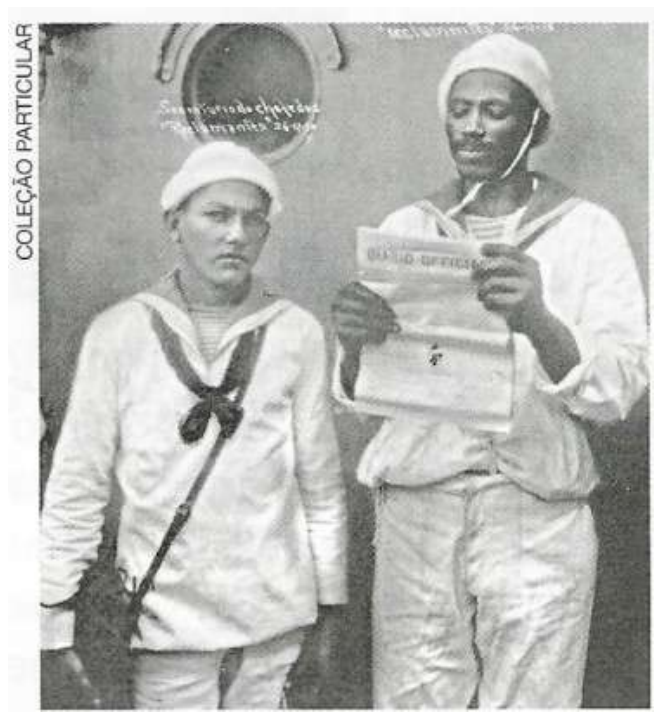
\includegraphics[width=\linewidth]{static/simulados/coluni/figuras/2026/questao-38/figura-1.png}
\end{minipage}

Sobre o movimento liderado por João Cândido e os motivos que levaram à sua eclosão, assinale a afirmativa CORRETA:\begin{enumerate}
\item Trata-se da Revolta da Chibata, que foi motivada, entre outros fatores, pela imposição de castigos corporais aos marinheiros e pelo descontentamento com os baixos soldos, a má alimentação e o trabalho excessivo.
\item Trata-se da Revolta da Vacina, causada pela indignação do povo com a criação de uma lei que determinava a vacinação obrigatória contra a varíola e que permitia, se necessário, o uso da força na aplicação da vacina.
\item Trata-se da Revolta dos 18 do Forte de Copacabana, que ocorreu em função da insatisfação de jovens oficiais do exército, que defendiam maior participação da instituição nas decisões políticas.
\item Trata-se da Revolta da Armada, que foi desencadeada pelo descontentamento de oficiais da Marinha que estavam insatisfeitos com a limitada participação dessa instituição na política brasileira.\end{enumerate}